\documentclass{article}

% Packages for setting up page margins
\usepackage[margin=1in]{geometry}

\usepackage{graphicx, setspace, amsmath, mathtools, amssymb, url, float, listings}
\setlength{\parskip}{2mm}
\graphicspath{ {./images/} }

% Title
\title{CS535 Design and Analysis of Algorithms - Midterm}
\author{Batkhishig Dulamsurankhor - A20543498}
\date{\today} % Use \date{} for no date

\begin{document}

\maketitle

\begin{enumerate}
  \item
  \begin{enumerate}
    \item For subset system $(E,\mathcal{I})$ to be a matroid, it must satsify the following three properties.
    Here I am making assumption that $|E|>0$ or the network $G$ has at least one edge.

    \begin{itemize}
      \item First, it has to be a finite and non-empty set. It is trivial and subsets are limited by $k$ number of edges.
      If we assume that $|E|>0$ meaning we have at least an edge in the network, this property is satisfied.
      \item The second is heredity property.
      In this network $G$, if a subset $S_1$ of $E$ is an independent set, then $S_2$ that is a subset of $S_1$ is also an independent set.
      In other words, $S_2\subset S_1$ and if $S_1\in \mathcal{I}$ then $S_2\in \mathcal{I}$.
      Let's say $k=1$, so we can have at most one element in a subset.
      We have an independent set $|S_1|=k$, so a proper subset of $S_1$ is $\{\varnothing\}$ and by definition we know it also a part of independent sets.
      Therefore, it does satisfy the second property.
      \item The third property is exchange property.
      As long as $k>0$, we can always find an independent set $E_1$ which has more elements than an independent set $E_2$.
      So by exchange property, $E_1,E_2\in\mathcal{I}$ and if $|E_1|>|E_2|$ then we can always find an edge $e\in E_1$ such that $E_2\cup\{e\}\in \mathcal{I}$.
      So, it does satisfy the third property.

    \end{itemize}
    $(E,\mathcal{I})$ is a matroid assuming that the network $G$ has at least one edge.

    \item For a subset system $(E,\mathcal{J})$ to be a matroid, it has to satisfy the following three properties.

    \begin{itemize}
      \item First, it has to be a finite and non-empty set.
      We know $E$ has at least $e_1$ and $e_2$, so it is non-empty.
      With finite number of edges $E$, the first property is satisfied.
      \item The second is heredity property.
      Heredity property defines that a subset of independent set is always an independent set.
      Let's say an independent set $E_1$ contains $e_1$ and not $e_2$.
      Then the subset of $E_1$, that is $E_2$, can contain $e_1$ but never $e_2$. If $e_1\in E_1$, $e_2\notin E_1$ and $E_2\subseteq E_1$ then $e_2\notin E_2$.
      In other words, $e_1$ and $e_2$ cannot be in the same independent set.
      This doesn't break the rule defined in the problem that $\mathcal{J}$ contains at most one of $e_1$ and $e_2$ and satisfies the heredity property.
      \item The third property is exchange property.
      Exchange property defines that for $E_1,E_2\in\mathcal{J}$, if $|E_1|>|E_2|$ then $\exists e\in E_1-E_2$ such that $E_2\cup\{e\}\in\mathcal{J}.$
      Let's provide a counter example that doesn't satisfy this property.
      Suppose we have independent sets $E_1=\{e_1,e_3\}$ and $E_2=\{e_2\}$ where $e_2$ and $e_3$ are dependent on each other.
      This satisfies the rule defined in the problem that $\mathcal{J}$ contains at most one of $e_1$ and $e_2$.
      By exchange property, there should be some element in $E_1$ such that adding it makes $E_2$ independent set.
      We know that $e_2$ and $e_3$ are dependent on each other, making $e_1$ the answer.
      However, we can have at most one of $e_1$ and $e_2$ in $\mathcal{J}$ and to satisfy exchange property, we have to break this rule.
      For this reason, it doesn't satisfy exchange property.
    \end{itemize}
    Therefore, $(E,\mathcal{J})$ doesn't form a matroid.
  \end{enumerate}
  \item Since technical analyst Dr. W.Ho. Cares's algorithm doesn't terminate after finding MST, we have to check all the other edges left in the graph.
  Because we found MST, we have only one set in our union find data structure where all vertices are in.
  So finding an edge always results in a cycle, or both vertices have the same ancestor.
  Also, it is given that Dr. W.Ho. Cares is using path compression making the union find data structure more efficient.

  I think remaining $O(m)$ finds take only $O(m)$ steps is true.
  An actual cost for find is the height of vertex $n_i$, $h(n_i)$.
  We can define potential function as the complexity of the set.
  It reduces everytime find operation is executed, because the tree is compressed and becomes flatter.
  By path compression, all vertices from $n_i$ up to the root is has to be connected to the root except from the upmost vertices that is already connected to the root.
  So the change in potential function becomes $-(h(n_i)-1)$.

  The following is an amortized cost of a single find operation:

  $AM_i=Actual_i+\Delta PF_i=h(n_i)+(-h(n_i)-1)=h(n_i)-h(n_i)+1=1$.

  So the total amortized cost is:

  $\sum_{i}^{m} AM_i = \sum_{i}^{m} Actual_i+\sum_{i}^{m} \Delta PF_i=m*1=m$

  Therefore, the remaining $O(m)$ finds takes $O(m)$ so Dr. W.Ho Cares's claim is true.

  \item In a normal Binomial heap, the number of nodes in a tree of rank $r$ is at most $2^r$.
  If we allow up to $k$ trees of any given rank, we can have $k+1$ number of trees of rank $r-1$ for the of rank $r$.
  This is true for $k=1$, the normal Binomial heap because a tree of a rank $r$ has $k+1=2$ trees of rank $r-1$.
  Let's say $k=2$, then a tree of a rank $r$ has $k+1=3$ trees of rank $r-1$.
  We can see the pattern here, so the number of nodes a modified Binomial heap that can have up to $k$ trees of a given rank is at most $(k+1)^r$.

  \begin{figure}[H]
    \centering
    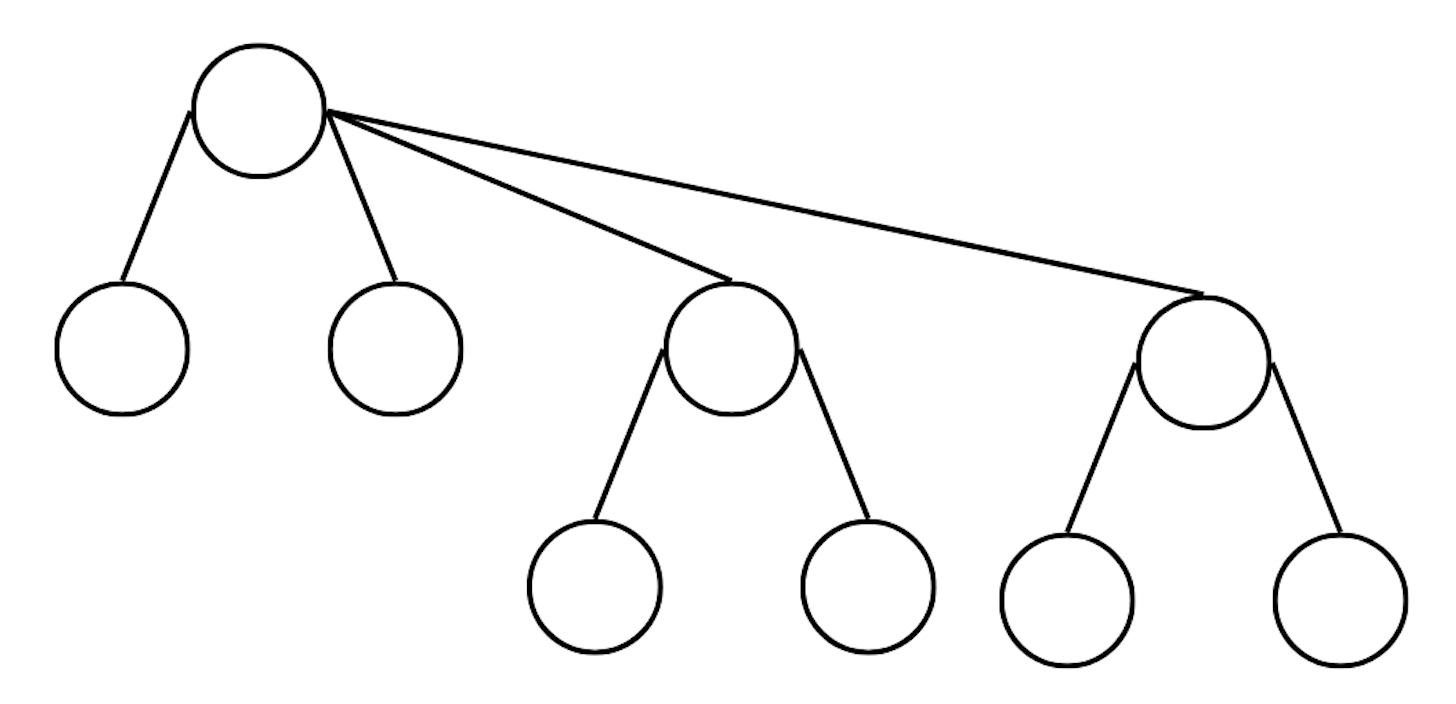
\includegraphics[width=0.5\textwidth]{image1.png}
    \begin{minipage}{0.5\textwidth}
        \centering
        Example: $k=2$, $r=2$ tree. We can count that the total number of nodes in this tree is $(k+1)^r=(2+1)^2=9.$
    \end{minipage}
  \end{figure}

  Insert operation has two parts. First, we insert the element to the forest, which is a constant time operation.
  Then we have to merge the trees with equal ranks, or to a tree with upper rank that has less than $k$ number of that rank tree.
  We have to repeat this process for higher rank trees if we have to.
  The merging two trees takes constant time. However in the worst case scenario, we will need to merge up to $log_{k+1}n$ number of trees.
  Worst case scenario is when adding a single node results in merging of trees for higher and higher ranks and eventually form a single tree.
  Therefore, the total time complexity is $O(insert+merge)=O(1+1*log_{k+1}n)=O(log_{k+1}n)$.

  For Deletemin operation, first we find the minimum value root among the trees.
  We know that there can be up to $log_{k+1}n$ number of trees in the heap, making this step $O(log_{k+1}n)$.
  Then, we remove the root and add the subtrees to the heap.
  Removing the root takes constant time.
  Finally, we have to merge the subtrees to the original heap, making no rank has more than $k$ trees.
  This step has similar complexity to the one we analyzed in insert operation.
  The time complexity for this step is also $O(log_{k+1}n)$.
  The total time complexity of deletemin operation is $O(findroot+removeroot+merge)=O(log_{k+1}n+1+log_{k+1}n)=O(log_{k+1}n)$.

  \item In this problem, we have one processor and need to minimize the averge finish time of jobs.
  Jobs have start time $s_j$ and duration $t_j$ and can be interrupted, meaning we can pause it and execute another job.

  Let's design an algorithm to find the optimal answer.
  The intuition is that we have to execute jobs that finishes the earliest.
  At any point when there is a new job or its start time hits, we add it to the pending jobs and get the earliest finishing job again.
  When a job finishes executing, we pick up the next job that finishes earliest.
  We keep doing this until no job is left for scheduling and end up with the optimal schedule.

  The following is the pseudocode for the algorithm:

  \begin{lstlisting}
    sort(H) by start_time;
    result;
    PriorityQueue pq on duration;
    
    while H has upcoming job:
      pq.add(H.next);
      
      while (H.next.start_time>current_time+pq.peek.duration):
        pq.poll();
        result.add(current_time);
    
    while pq is not empty:
      pq.poll();
      result.add(current_time);
    
    return avg(result);

  \end{lstlisting}

  To efficiently calculate and find the next earliest finishing job, I have used priority queue/heap.
  Let's analyze the time complexity.
  First we have to sort jobs by their start time, which takes $O(nlogn)$.
  Next, for each job, we have to insert it to the priority queue by their remaining duration (we can calculate relative duration by simply keeping current time in a constant time).
  Since insert in heap is $O(logn)$, this step takes $O(nlogn)$.
  During the process, we also have to execute deletemin to remove jobs from priority queue, and add it to the result.
  The time complexity for deletemin is $O(logn)$, adding deleted element is $O(1)$ and we have execute this by the number of jobs $n$, thus $O(nlog(n+1))$.
  Finally, calculating the average and returning result takes constant time $O(1)$.

  The time complexity of the algorithm:

  $O(sorting+insert+deletemin+average)=O(nlogn+nlogn+nlogn+1)=O(nlogn)$

  Let's prove the correctness of this algorithm by contradiction.
  Let's assume that our algorithm resulted in schedule $S$, and there exist another schedule $S^\prime$ such that the average finish time $S^\prime$ is smaller than $S$'s.
  This claim suggests that at some point in $t$, the schedule $S^\prime$ is running job $j_m$ that has more remaining duration than job $j_n$.

  $\Delta t=t_m-t_n$.

  The finish time of $j_m$ is $t_m$, but finish time of $j_n$ will be at least $t_m+t_n$.
  The total of their finish time becomes $T^\prime_{mn}=t_m+t_m+t_n$.
  However, by swapping these two jobs we have less total time $T_{mn}=t_n+t_n+t_m$, efficient by $\Delta t$.
  This makes the average finishing time of $S^\prime$ greater than $S$, contradicting the claim.
  Therefore, this algorithm is correct.
\end{enumerate}


\end{document}